\begin{figure}[htbp]
\centering
\begin{tikzpicture}[x=1cm,y=1cm]
\node[anchor=south west,inner sep=0] at (0,0) {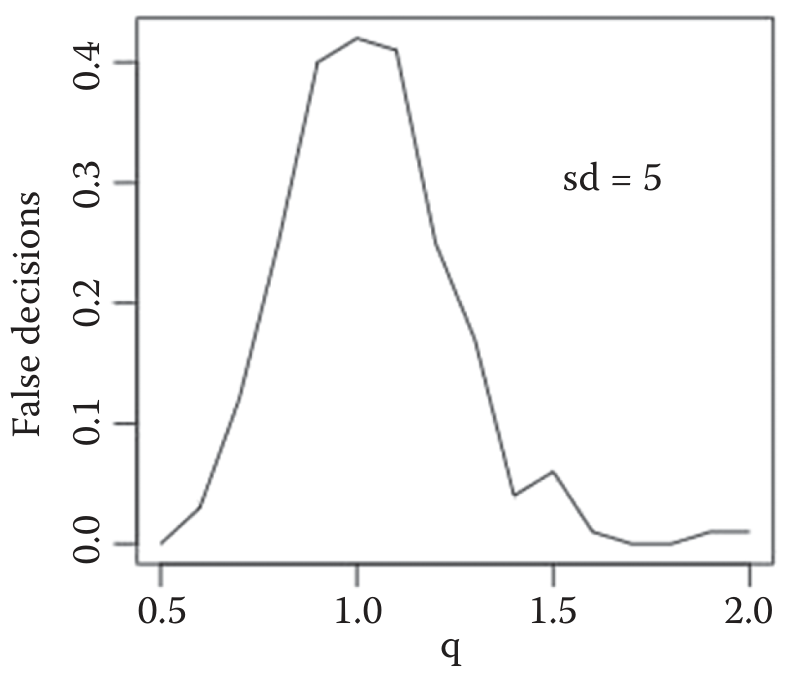
\includegraphics[width=9.5cm]{figures/ch04a_fig24_data.png}};
\fill[white] (0.0824,2.9062) rectangle (0.6164,5.9451);
\node[inner sep=0pt,fill=white,rotate=90,font=\fontsize{8}{8}\selectfont] at (0.3494,4.4257) {误判率};
\fill[white] (6.7848,5.7832) rectangle (8.0425,6.3172);
\node[inner sep=0pt,fill=white,rotate=0,font=\fontsize{8}{8}\selectfont] at (7.4137,6.0502) {标准差=5};
\end{tikzpicture}
\origfig{24}{假定线性模型及非正态误差分布时，双变量因果发现的误判率。}
\label{fig:ch04a-24}
\end{figure}
